%use in documents with \subfile{tex/intro}
\documentclass[../../master.tex]{subfiles}

\begin{document}

\subsection{\texttt{ASPRAlign}}
\label{sub:appendix:aspra}

Initially, \texttt{ASPRAlign} was evaluated as an example for a tree alignment distance on RNA secondary structures with pseudoknots \parencite{quadrini_algebraic_2019}.

A simplified version of the rewriting rules of the tree grammar described in \parencite{quadrini_algebraic_2019} is displayed in \eqref{eq:methods:treegrammar}.

\begin{align}\label{eq:methods:treegrammar}
	\begin{split}
		S \rightarrow &\leftrightarrows(\eta_1, T, \eta_2) \\
		T \rightarrow &\odot(T, (\odot, \eta), C) \mid C \\ 
		C \rightarrow &\bowtie(C, (\bowtie, k), I) \mid N \\
		N \rightarrow &\Cap(T, (\Cap, k), I) \mid I \\
		I \rightarrow & H (x_1 \omega x_2)
	\end{split}
\end{align}

Using these rules, secondary structures with pseudoknots can be derived while simultaneously constructing a tree representation.

Without going too much into details, this procedure starts by truncating ($\leftrightarrows$) unpaired subsequences $\eta_1, \eta_2$ from a general \textit{pseudoloop}, i.e. a substructure $T$. $T$ may be rewritten as a concatenation $\odot$ of a similar pseudoloop and another type of pseudoloop $C$, where $\eta$ denotes an unpaired region between those two, or as a single pseudoloop $C$.
Similarly, $C$ may be rewriten as a crossing $\bowtie$  of a pseudoloop and a single hairpin $I$ containing paired symbols $x_1, x_2$ and an unpaired region $\omega$, or some nested loops $N$.
Finally, $N$ is rewritten as a nesting $\Cap$ of a general pseudoloop $T$ and a hairpin or just a single hairpin.
Note that $k$ is used to track the start position of the second argument of either $\bowtie$ or $\Cap$. 

Aligning two structures would be done based on their (\textit{algebraic}) trees node labels containing information about the operators used to derive them from this grammar.
This is done by constructing a \textit{structural} tree from the algebraic tree. An example of this is shown in Fig. \ref{fig:tset}.

\begin{figure}[!ht]
	\centering
	\begin{subfigure}[t]{0.3\textwidth}
		%\centering
		\begin{minipage}[b][4cm][c]{0.3\textwidth}
			\small
			\begin{verbatim}				
				...((...)...[...)...]...
				CCCUUAAUAGGGGAUAAUCCCGCC
			\end{verbatim}
		\end{minipage}
		\caption{Secondary structure with a compatible RNA sequence in dot-bracket notation.
		}\label{fig:tset:a}
	\end{subfigure}%
	\begin{subfigure}[t]{0.4\textwidth}
		\centering
		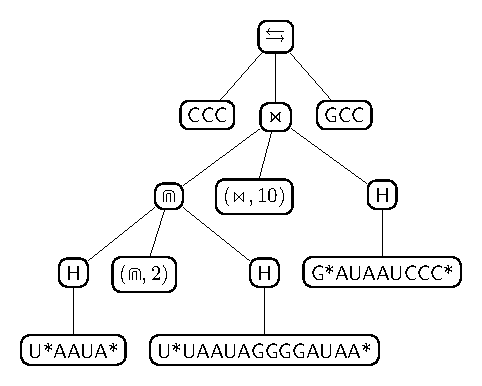
\includegraphics[width=\textwidth]{pic/results/aspratree/tset.pdf}
		\caption{\textit{Algebraic} RNA tree as derived from \autoref{fig:tset:a} using \eqref{eq:methods:treegrammar}.
		}\label{fig:tset:b}
	\end{subfigure}
	\begin{subfigure}[t]{0.28\textwidth}
		\centering
		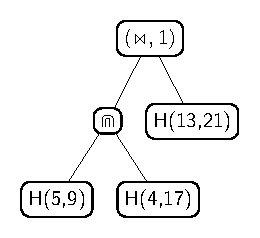
\includegraphics[width=\textwidth]{pic/results/aspratree/tset_struct.pdf}
		\caption{\textit{Structural} RNA tree constructed from \ref{fig:tset:b}.
		}\label{fig:tset:c}
	\end{subfigure}
	\caption[Structure Trees as used in \texttt{APSRAlign}]{
		\begin{enumerate*}[label={(\alph*)}, font={\bfseries}]
			\item A small pseudoknotted RNA secondary structure and
			\item the algebraic RNA tree obtained from the grammar rules in \eqref{eq:methods:treegrammar} as described in \parencite{quadrini_algebraic_2019}. Note that the integer in the leaf $(\bowtie, 10)$ is an instance of $k$ as in \eqref{eq:methods:treegrammar}.
			\item The structural RNA tree. The integer in the root $(\bowtie, 1)$ is different to \autoref{fig:tset:b} and denotes the number involved base pair crossings. 
		\end{enumerate*}
	}\label{fig:tset}
\end{figure}

A measure of similarity between structural trees is computed by scoring insertion, deletion or replacement of tree nodes containing the operators used in the grammar and finding an alignment that minimizes this score.

For reference, \autoref{eq:methods:scoring} lists the original scoring function used in \parencite{quadrini_algebraic_2019} and the actual values used as constants.

\begin{equation}\label{eq:methods:scoring}
	\begin{aligned}
		&\sigma_s((\bowtie, h), (\bowtie(h'))) = c_{\mathrm{m}} \cdot |h - h'| & c_{\mathrm{m}} &= 0.01 \\
		&\sigma_s(op_1, op_2) = o_{\mathrm{r}} & o_{\mathrm{r}} &= 1  \\
		&\sigma_s(op, -) = \sigma_s(-, op) = o_{\mathrm{di}} & o_{\mathrm{di}} &= 1 \\
		&\sigma_s(H(i, j), H(i', j')) = 0 &  & \\
		&\sigma_s(H(i, j), op) = \sigma_s(op, H(i, j)) = +\infty & & \\
		&\sigma_s(H(i, j), -) = \sigma_s(-, H(i, j)) = h_{\mathrm{di}} & h_{\mathrm{di}} &= 1
	\end{aligned}
\end{equation}

where $op \in \{(\bowtie, h), \Cap, \odot\}$.

In Addition, in this work, the scoring function was modified as written in \autoref{eq:methods:scoringmod} to achieve more fine-grained structure comparisons.

\begin{equation}\label{eq:methods:scoringmod}
	\begin{aligned}
		&\sigma_s(op, -) = \sigma_s(-, op) = o_{\mathrm{di}} & o_{\mathrm{di}} &= 0 \\
		&\sigma_s(H(i, j), H(i', j')) = |i - i'| + |j - j'| &  & \\
	\end{aligned}
\end{equation}

With the modifications in \autoref{eq:methods:scoringmod}, the cost of inserting or deleting an operator was removed since this coincides with inserting or deleting a hairpin using the tree grammar rules \eqref{eq:methods:treegrammar}.
Additionally, hairpin mismatches were penalized by the difference of their indices.
\todo{this is ok here since we have always constant sequence length. a coarse-grained tree alignment does make sense for different lengths}

\todo{shortcomings of ASPRAdistance (i.e. speed, not a metric, didn't consider open chain, no proofs about uniqueness of decomposition?, actual grammar implemented in \texttt{ASPRATree.java} differs from paper)}

\subsubsection{Comparison to Base Pair Distance}
\label{sub:appendix:strcomp}

\begin{figure}[!ht]
	\centering
	\begin{subfigure}[t]{0.5\textwidth}
		\centering
		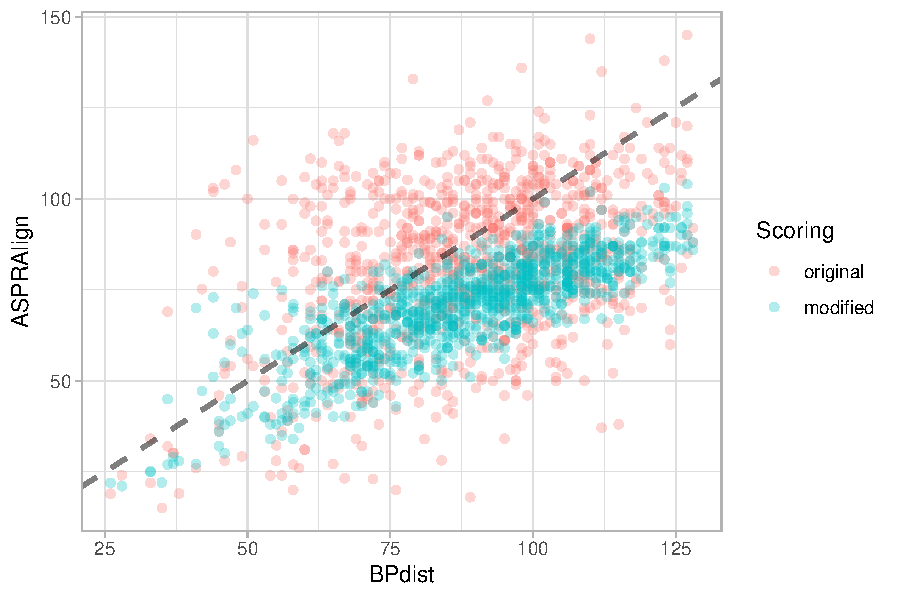
\includegraphics[width=\textwidth]{pic/results/aspratest_comp_random.pdf}
		\caption{Structures were predicted using \texttt{pKiss} using uniformly sampled sequences compatible to the target structure.
		}\label{fig:distcomp:a}
	\end{subfigure}%
	\begin{subfigure}[t]{0.5\textwidth}
		\centering
		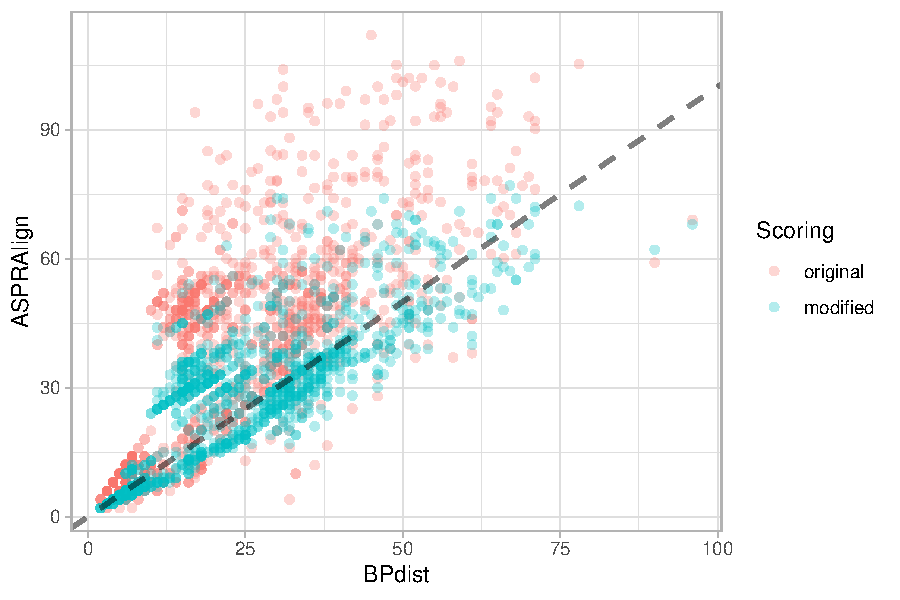
\includegraphics[width=\textwidth]{pic/results/aspratest_comp_allconstraints.pdf}
		\caption{Structures were used from later generated sequence designs.
		}\label{fig:distcomp:b}
	\end{subfigure}
	\caption[Structure Distance Measure Comparison]{Comparison of \texttt{ASPRAlign} with the usual base-pair distance (including pseudoknots). Additionally to the original scoring function of \texttt{ASPRAlign}, the scoring was modified as specified in \autoref{eq:methods:scoringmod} and added to the comparison. Length of the structures used was $N = 197$. All distances were calculated relative to the truncated structure in \autoref{fig:azodata:b}.
	}\label{fig:distcomp}
\end{figure}

\begin{figure}[!ht]
	\centering
	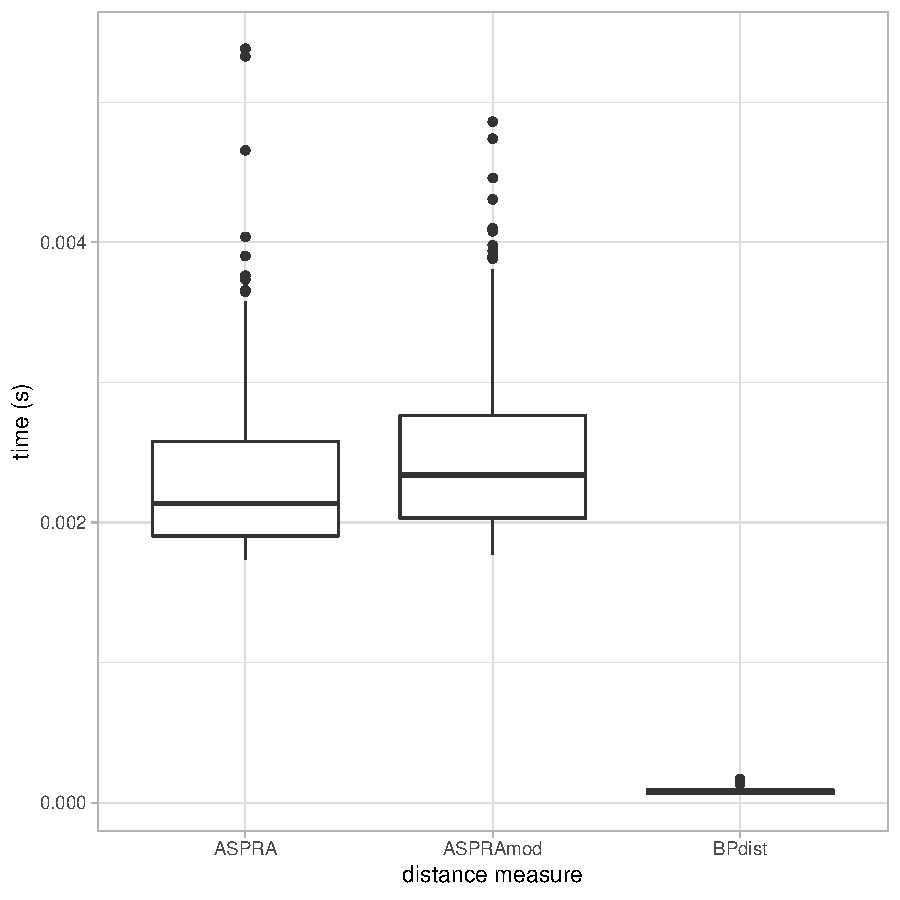
\includegraphics[width=0.4\textwidth]{pic/results/aspratest_allconstraints_time.pdf}
	\caption[Structure Distance Measure Runtime]{Runtime Comparison of \texttt{ASPRAlign} with the usual base-pair distance (including pseudoknots). Additionally to the original scoring function of \texttt{ASPRAlign}, the scoring was modified as specified in \autoref{eq:methods:scoringmod} and added to the comparison. Length of the structures used was $N=197$.
	}\label{fig:distruntime}
\end{figure}

\begin{figure}[!ht]
	\centering
	\begin{subfigure}[t]{0.4\textwidth}
		%\centering
		\begin{minipage}[b][6cm][c]{0.4\textwidth}
			\large
			\begin{verbatim}		
				...[...(...]...(...))...
				AUAAGCGAUCCUCCUCGCAGUAAA
			\end{verbatim}
		\end{minipage}
		\caption{Secondary structure with a compatible RNA sequence in dot-bracket notation.
		}\label{fig:test:a}
	\end{subfigure}%
	\begin{subfigure}[t]{0.6\textwidth}
		\centering
		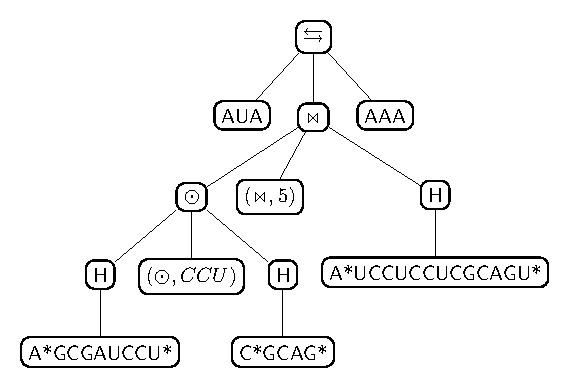
\includegraphics[width=\textwidth]{pic/results/aspratree/test.pdf}
		\caption{\textit{Algebraic} RNA tree as produced from \autoref{fig:test:a} using \texttt{ASPRAlign}.
		}\label{fig:test:b}
	\end{subfigure}
	\caption[Structure Counter Example for \texttt{APSRAlign}]{
		\begin{enumerate*}[label={(\alph*)}, font={\bfseries}]
			\item A small pseudoknotted RNA secondary structure and
			\item its algebraic RNA tree obtained using \texttt{ASPRAlign}. Note that this structure is the exact reverse of the structure in \autoref{fig:test:a} and violates $C$-rewriting of the grammar \eqref{eq:methods:treegrammar}.
		\end{enumerate*}
	}\label{fig:test}
\end{figure}

A transcript of the actual tree grammar implemented in \texttt{ASPRAlign} \todo{properly refer to \texttt{ASPRATree.java}??}
is given in \eqref{eq:results:actualtreegrammar}.
In this grammar, the structure in \autoref{fig:test:a} can be derived.

\begin{align}\label{eq:results:actualtreegrammar}
	\begin{split}
		S \rightarrow &\leftrightarrows(\eta_1, N, \eta_2) \mid \leftrightarrows(\eta_1, N, \eta_2) \\
		N \rightarrow &\Cap(S, (\Cap, k), I) \mid I \\
		T \rightarrow &\bowtie(S, (\bowtie, k), I) \mid \odot(S, (\odot, \eta), S) \\ 
		I \rightarrow & H (x_1 \omega x_2)
	\end{split}
\end{align}

However, neither grammar \eqref{eq:methods:treegrammar} nor \eqref{eq:results:actualtreegrammar} can derive the open chain structure.

Given a palindromic structure such as \texttt{(........(.....).......)}, chiral structures like those in \autoref{fig:tset:a} and \autoref{fig:test:a} would be expected to have equal distance scores to the palindrome. 
With grammar \eqref{eq:results:actualtreegrammar} and the default scoring parameters of \texttt{ASPRAlign}, this is not the case.
\todo{more context. rather discussion? display actual values in a table}

\end{document}
